\chapter{Prezentacja działania aplikacji}
\label{cha:prezentacja}

W tej części pracy znajduje się opis aplikacji widzianej oczami użytkownika. W rozdziale~\ref{sec:interfejsUzytkownika} został
przedstawiony interfejs graficzny użytkownika. Następnie rozdział~\ref{sec:praktyczneUzycieSystemu} prezentuje działanie aplikacji wykorzystując przykładowe dane hospitalizacji. W rozdziale tym znajduje się opis praktycznego użycia systemu dla realnych danych. Sekcja~\ref{sec:testyIntegracyjne} zawiera przykładowy test integracyjny jednej ze ścieżek poszukiwania rozwiązania.

%---------------------------------------------------------------------------

\section{Interfejs użytkownika}
\label{sec:interfejsUzytkownika}
Aplikacja posiada standardowo okienkowy interfejs użytkownika. Skórka aplikacji jest ustawiona na przyjazny ,,PlasticXPLookAndFeel''.

Wszystkie funkcjonalności, takie jak dodawanie, usuwanie, filtrowanie oraz cały widoczny układ komponentów graficznych dostarcza framework Valkyrie-RCP. Realizuje je klasa ,,DataEditor'', która jest komponentem graficznym(Widgetem). Do obiektu klasy ,,DataEditor'' wstrzykiwane są JavaBean'y: \textbf{DataProvider} - fasada danych dla interfejsu użytkownika, \textbf{DetailForm} - forma do dodawania/usuwania danych, \textbf{FilterForm} forma dla dodatkowego filtrowania oraz \textbf{TableWidget} - obiekt definiujący wyświetlaną tabelkę danych\cite{valkyrie_reference}.
Rysunek \ref{img:patient} ilutruje widok bazy pacjetnów, który jest oparty na szablonie ,,DataEditor''.

\begin{figure}[!ht]
\centering
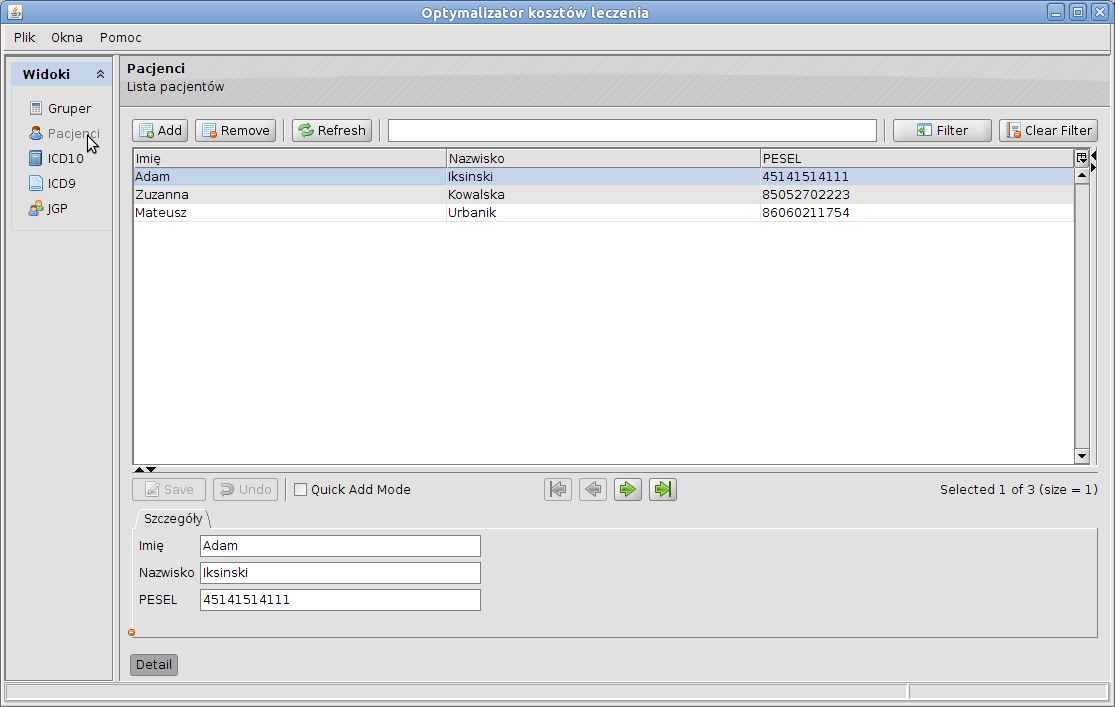
\includegraphics[scale=0.4]{images/patient} 
\caption[Widok bazy pacjentów]{Widok bazy pacjentów.}
\label{img:patient}
\end{figure}

W oparciu o wzorzec ,,DataEditor'' zbudowane są następujące widoki: katalog kodów \mbox{ICD-9}, \mbox{ICD-10}, JGP. Z tą różnicą w~stosunku do widoku bazy pacjentów, że zablokowana jest dla nich możliwość dodawania, edycji i~usuwania.

%---------------------------------------------------------------------------

\section{Praktyczne użycie systemu}
\label{sec:praktyczneUzycieSystemu}
Aby zilustrować działanie aplikacji przedstawiono w~tym podrozdziale konkretny i~realny przypadek użycia aplikacji. Zostanie wykorzystany również mechanizm dzięki, któremu lekarz ma możliwość optymalizacji kosztów leczenia pacjenta.

Zdefiniowano fakty wejściowe. Leczony pacjent urodzony w~1937 roku ma 75 lat, jest mężczyzną, przyjęty był na okres 7 dni w~trybie przyjęcia ,,Przyjęcie planowe na podstawie skierowania'' oraz wypisany trybie ,,Zakończenie procesu terapeutycznego lub diagnostycznego''. Typ hospitalizacji ustalono na ,,Hospitalizacja zwykła''. Rysunek \ref{img:gruper1} przedstawia uzupełniony powyższymi danymi widok ,,Grupera''. 
Następnie należy zdefiniować pobyt. Do tego celu służy okno dialowe(Rys.~\ref{img:gruper2}) wyświetlane po kliknięciu przycisku ,,Dodaj pobyt''. Ustalono następujące dane pobytu: oddział, kod świadczenia. Data przyjęcia i~wypisu przepisuje się automatycznie.
Kolejnym krokiem jest dodanie zdiagnozowanych rozpoznań(Rys.~\ref{img:gruper3}). Aby dodać rozpoznanie do pobytu należy kliknąć przycisk ,,Select''.
Następnie dodano wykonane procedury medyczne. W tym celu należy kliknąć przycisk ,,Dodaj procedurę''(Rys~\ref{img:gruper5}).
Po wybraniu procedury należy ustalić w~jakim terminie została ona wykonana oraz ile razy(Rys.~\ref{img:gruper6}).
Zatwierdzenie przyciskiem ,,OK'' przenosi użytkownika do okienka z~zdefiniowanym pobytem(Rys.~\ref{img:gruper7}).
Kiedy wszystkie dane dla pobytu zostały uzupełnione, zapis pobytu następuje po zatwierdzeniu przyciskiem OK(Rys.~\ref{img:gruper7}).
Widok ,,Gruper'' z~wypełnionymi wszystkimi danymi wejściowymi prawidłowo pozwala użytkownikowi na uruchomienie algorytmu. Należy nacisnąć przycisk ,,Grupuj''(Rys.~\ref{img:gruper8}).

\begin{figure}%[!ht]
\centering
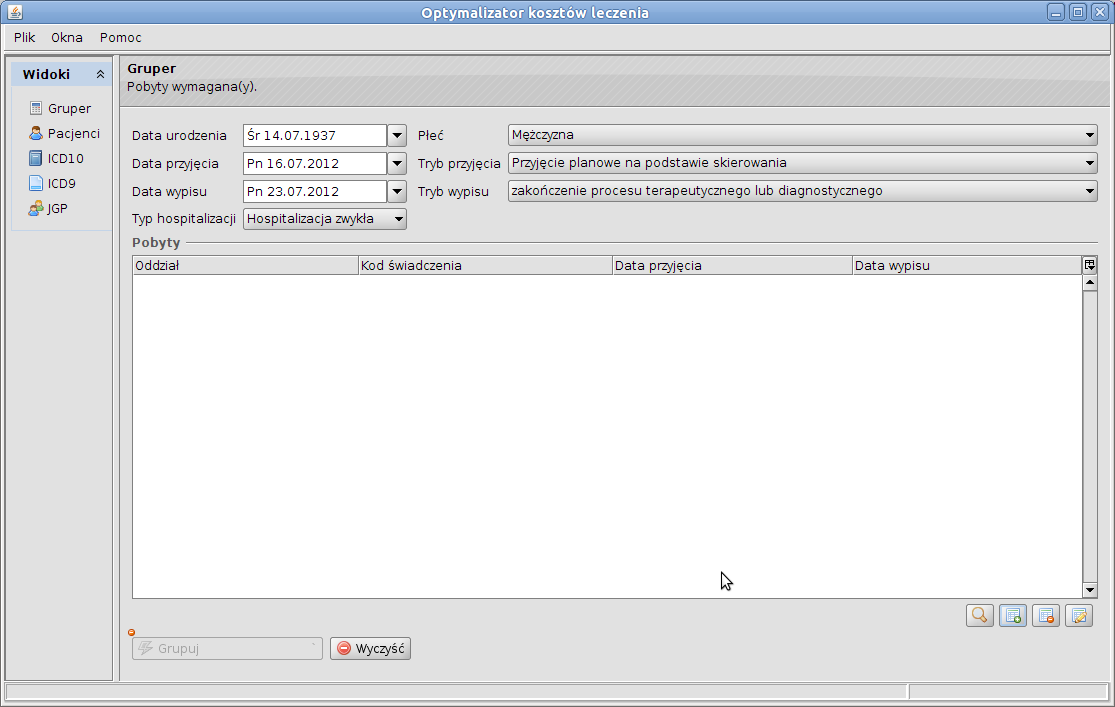
\includegraphics[scale=0.4]{images/gruper1}
\caption[Widok grupera]{Widok grupera - dane wejściowe.}
\label{img:gruper1}
\end{figure}

\begin{figure}%[!ht]
\centering
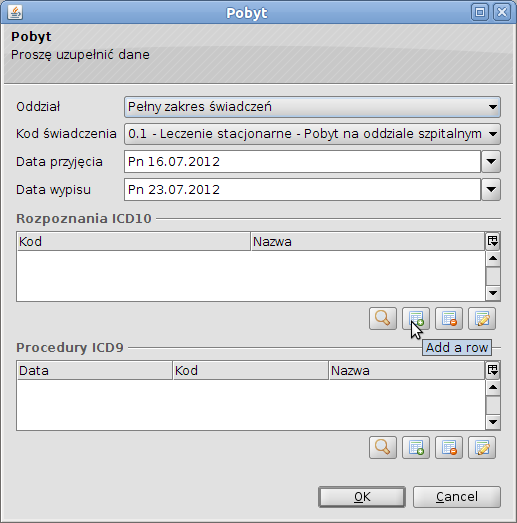
\includegraphics[scale=0.4]{images/gruper2}
\caption[Widok grupera]{Okno dialogowe - dodawanie pobytu.}
\label{img:gruper2}
\end{figure}

\begin{figure}%[!ht]
\centering
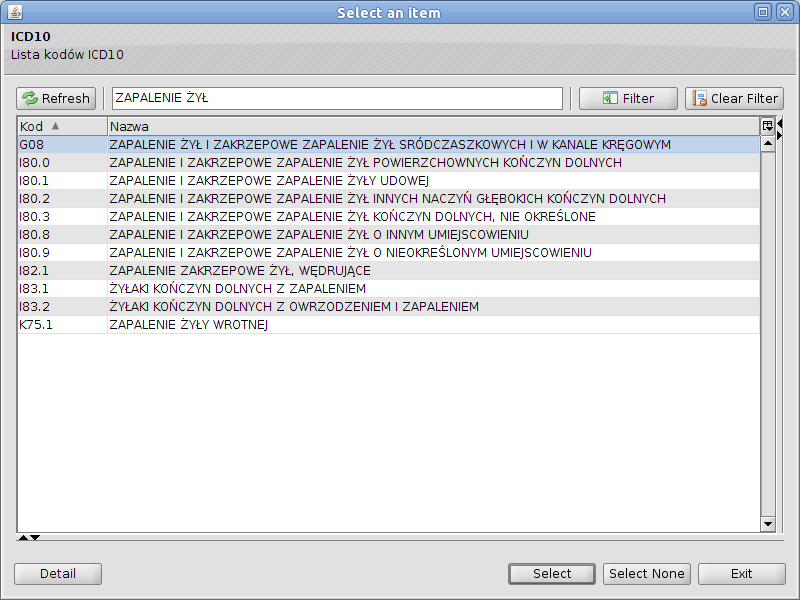
\includegraphics[scale=0.4]{images/gruper3}
\caption[Widok grupera]{Okno dialogowe - wybór rozpoznania.}
\label{img:gruper3}
\end{figure}

\begin{figure}%[!ht]
\centering
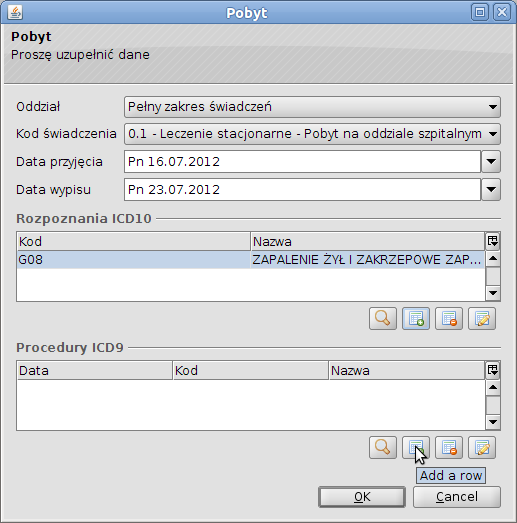
\includegraphics[scale=0.4]{images/gruper4}
\caption[Widok grupera]{Okno dialogowe - dodawanie pobytu - rozpoznanie.}
\label{img:gruper4}
\end{figure}

\begin{figure}%[!ht]
\centering
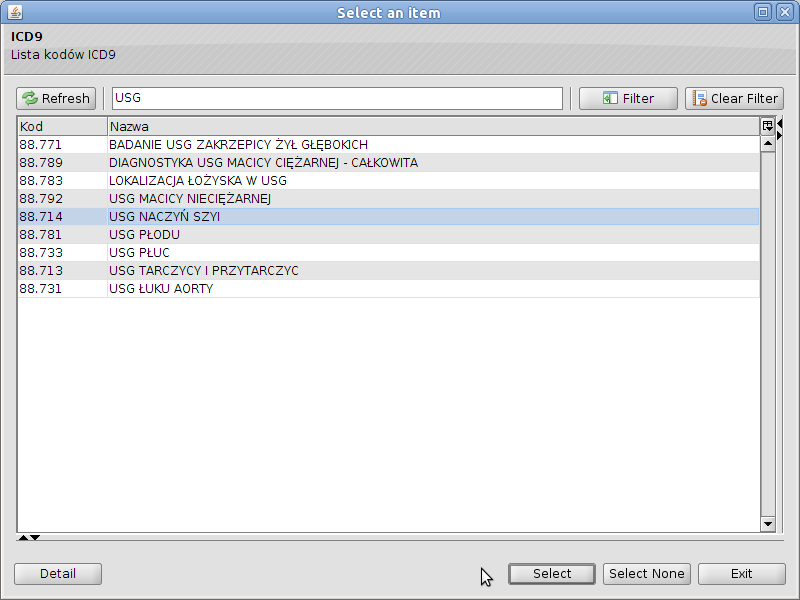
\includegraphics[scale=0.4]{images/gruper5}
\caption[Widok grupera]{Okno dialogowe - wybór procedury.}
\label{img:gruper5}
\end{figure}

\begin{figure}%[!ht]
\centering
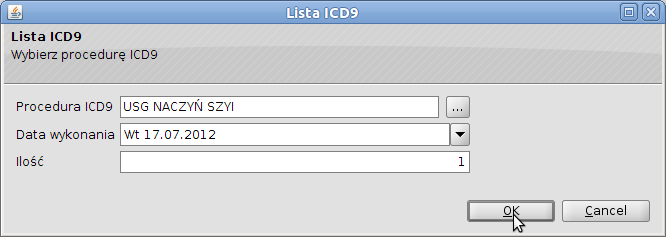
\includegraphics[scale=0.4]{images/gruper6}
\caption[Widok grupera]{Okno dialogowe - wybór procedury - data wykonania, ilość.}
\label{img:gruper6}
\end{figure}

\begin{figure}%[!ht]
\centering
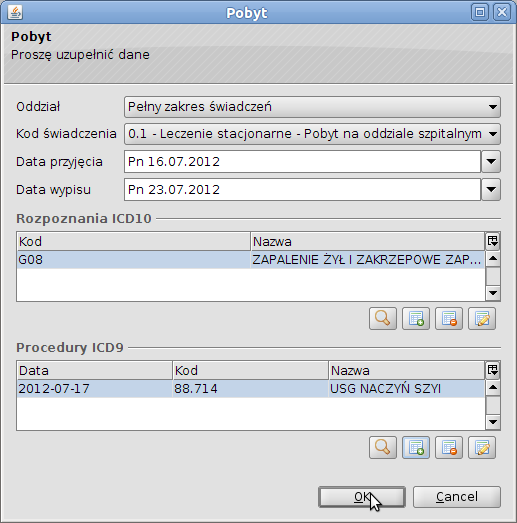
\includegraphics[scale=0.4]{images/gruper7}
\caption[Widok grupera]{Okno dialogowe - dodawanie pobytu - uzupełnione procedury i~rozpoznania.}
\label{img:gruper7}
\end{figure}

\begin{figure}%[!ht]
\centering
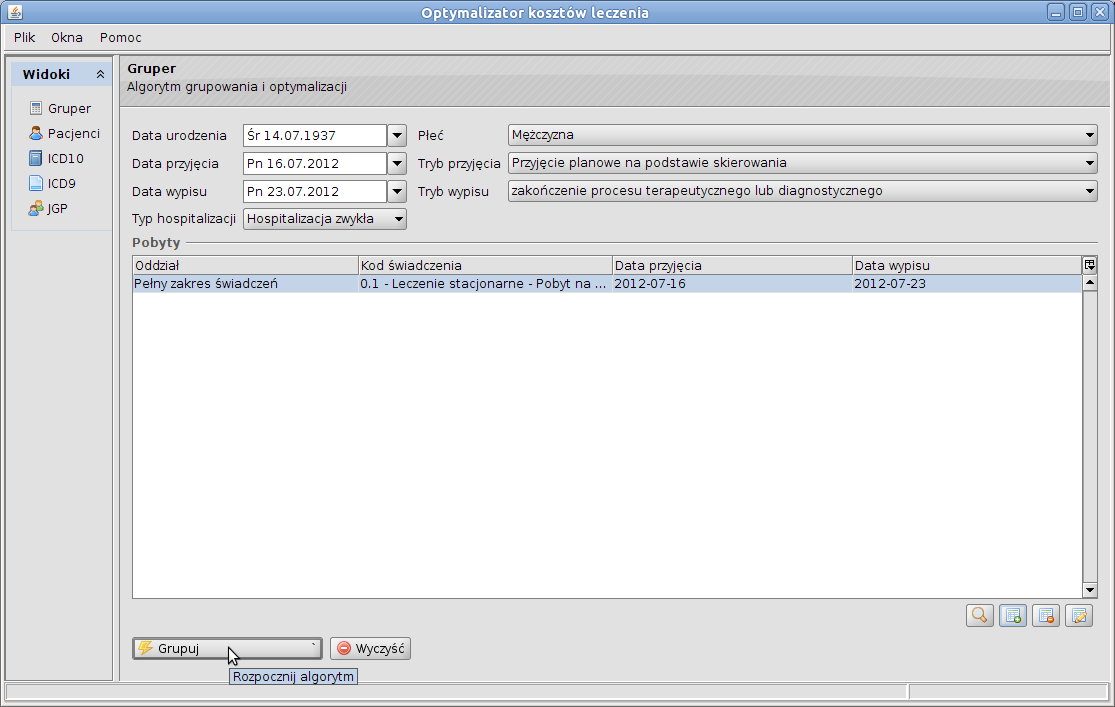
\includegraphics[scale=0.4]{images/gruper8}
\caption[Widok grupera]{Okno dialogowe - dodawanie pobytu - rozpoznanie.}
\label{img:gruper8}
\end{figure}

\begin{figure}%[!ht]
\centering
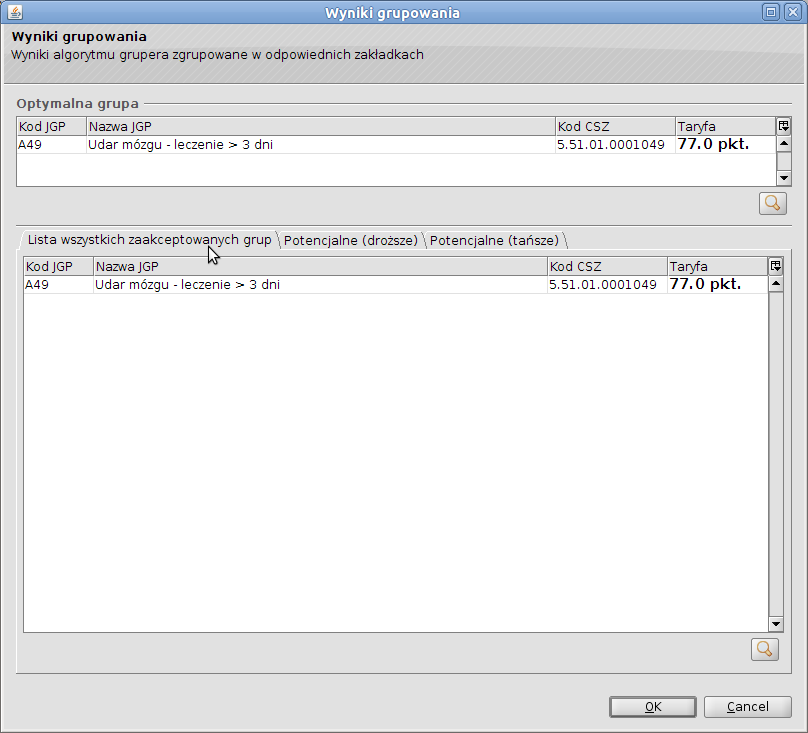
\includegraphics[scale=0.4]{images/gruper9}
\caption[Widok grupera]{Wyniki grupowania - Lista wszystkich zaakceptowanych grup.}
\label{img:gruper9}
\end{figure}

Uruchamiany jest algorytm wnioskowania, który wybiera warunki do sprawdzenia, testuje je, a~wyniki zapisuje na listach: Zaakceptowane, Potencjalnie droższe, Potencjalnie tańsze. W tym miejscu można zakończyć przebieg grupowania. Została wybrana optymalna grupa JGP: ,,A49 - Udar mózgu - leczenie > 3 dni'' oraz ustalona została wartość kosztów leczenia 77pkt(Rys.~\ref{img:gruper9}).

Następny krok w~prezentacji działania aplikacji to optymalizacja kosztów leczenia. Przedstawione zostanie narzędzie pozwalające przewidywać wyliczane według NFZ koszty leczenia pacjenta. Przeprowadzony zostanie proces maksymalizacji kosztów leczenia. Na tym etapie należy spojrzeć na zakładkę ,,Potencjalnie droższe''(Rys.~\ref{img:gruper10}). Znajdują się tu grupy JGP, wśród których poszukiwane jest najlepsze rozwiązanie.

\begin{figure}%[!ht]
\centering
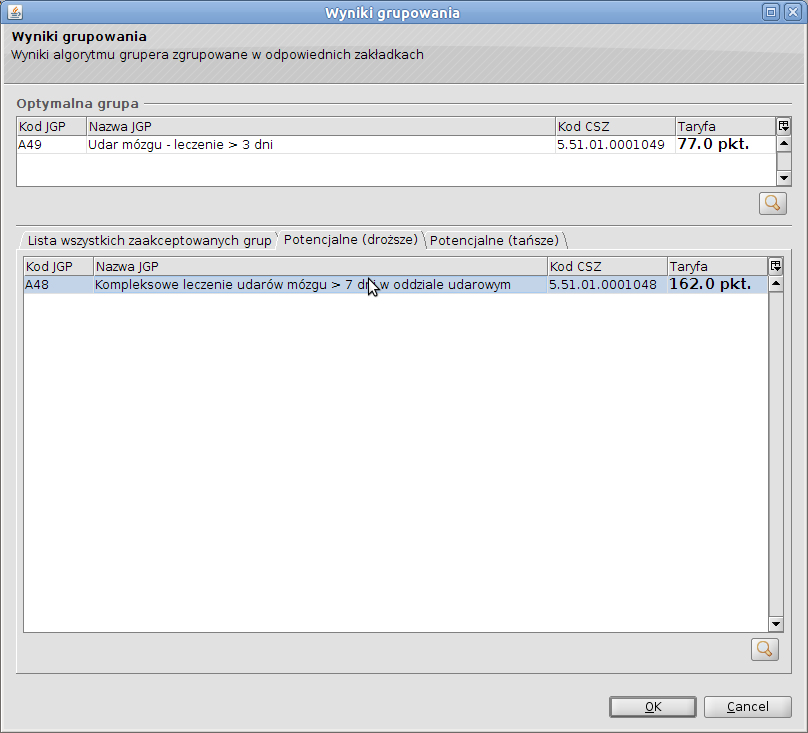
\includegraphics[scale=0.4]{images/gruper10}
\caption[Widok grupera]{Wyniki grupowania - Potencjalne (droższe).}
\label{img:gruper10}
\end{figure}

Zauważono, że istnieje grupa JGP dająca możliwość wygenerwoania kosztów w~wysokości 162pkt. Jest to ponad dwukrotnie większa wartość od wyliczonej aktualnie. Należy kliknąć przycisk ,,Szczegóły'' i~sprawdzić powody niezaakceptowania grupy A48(Rys.~\ref{img:gruper11}).

\begin{figure}%[!ht]
\centering
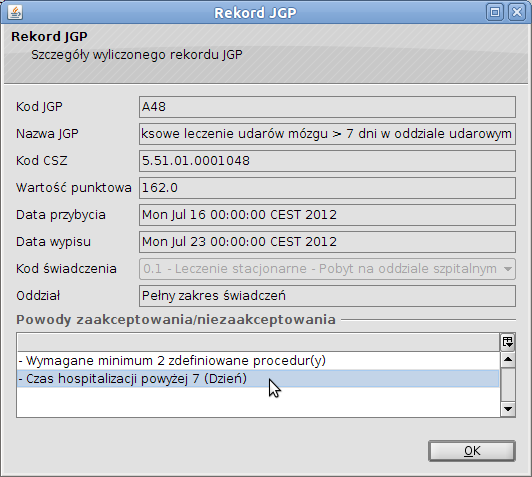
\includegraphics[scale=0.4]{images/gruper11}
\caption[Widok grupera]{Szczegóły niezaakceptowania grupy JGP.}
\label{img:gruper11}
\end{figure}

Z rysunku \ref{img:gruper11} można odczytać następujące powody niezaakceptowania pacjenta:
\begin{itemize}
 \item Wymagane jest zdefiniowanie 2 procedur medycznych,
 \item Wymagany jest czas hospitalizacji powyżej 7 dni.
\end{itemize}

W tym momencie zakres działania aplikacji się kończy. Jest to system doradczy, a decyzję optymalizacyjną podejmuje lekarz. Dla przedstawionego przypadku leczenia lekarz stwierdza, że przedłużenie pobytu na oddziale pacjenta o 1 dzień i~wykonanie dodatkowego badania podwoi koszty leczenia. W tym przypadku lekarz może podjąć decyzję o przedłużeniu leczenia o 1 dzień(Rys.~\ref{img:gruper12}).

\begin{figure}%[!ht]
\centering
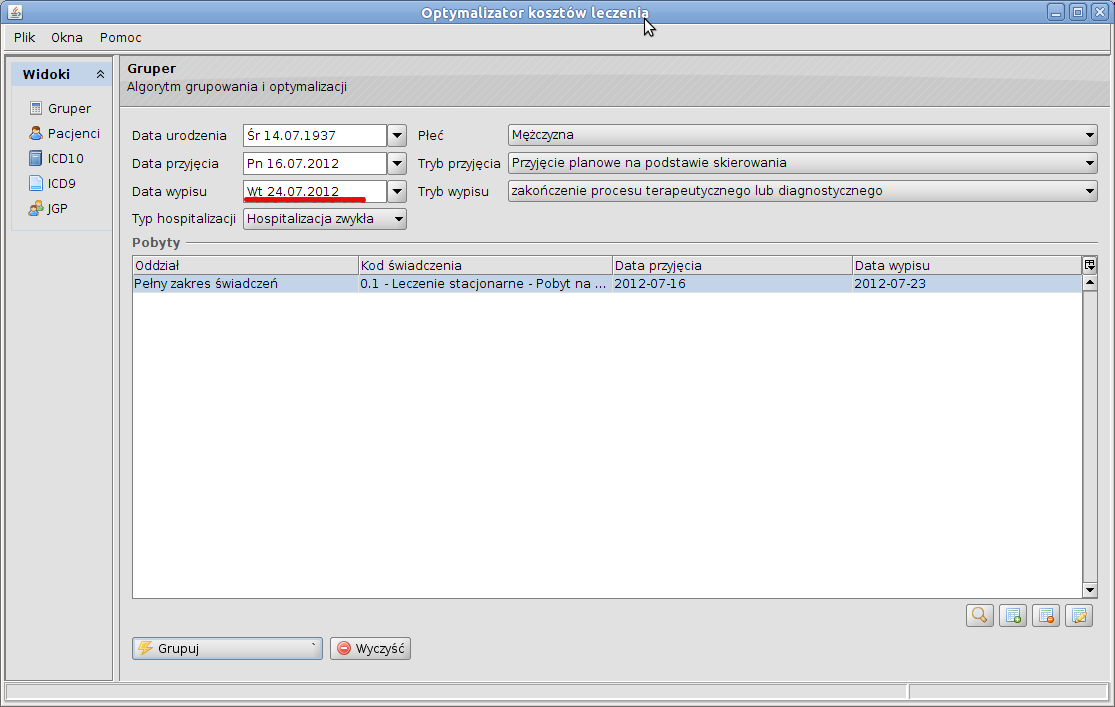
\includegraphics[scale=0.4]{images/gruper12}
\caption[Widok grupera]{Widok grupera - poprawione dane wejściowe.}
\label{img:gruper12}
\end{figure}

Dodano kolejną procedurę medyczną, badanie radiologiczne: ,,Arteriografia tętnicy szyjnej wewnętrznej''(Rys.~\ref{img:gruper13}, Rys.~\ref{img:gruper14}).

\begin{figure}%[!ht]
\centering
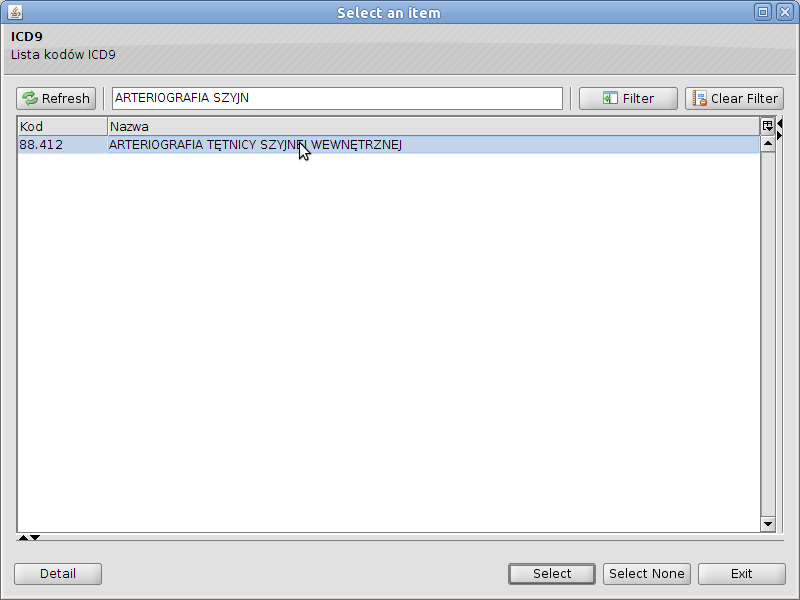
\includegraphics[scale=0.4]{images/gruper13}
\caption[Widok grupera]{Okno dialogowe - dodawanie procedury.}
\label{img:gruper13}
\end{figure}

\begin{figure}[!ht]
\centering
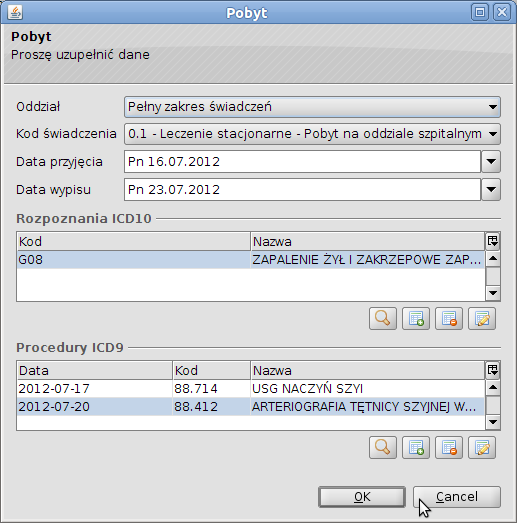
\includegraphics[scale=0.4]{images/gruper14}
\caption[Widok grupera]{Okno dialogowe - dodawanie pobytu - dodatkowo procedura.}
\label{img:gruper14}
\end{figure}

W wyniku ponownego uruchomienia algorytmu grupowania, otrzymano jako wynik spodziewaną grupę JGP(Rys.~\ref{img:gruper15}).

\begin{figure}%[!ht]
\centering
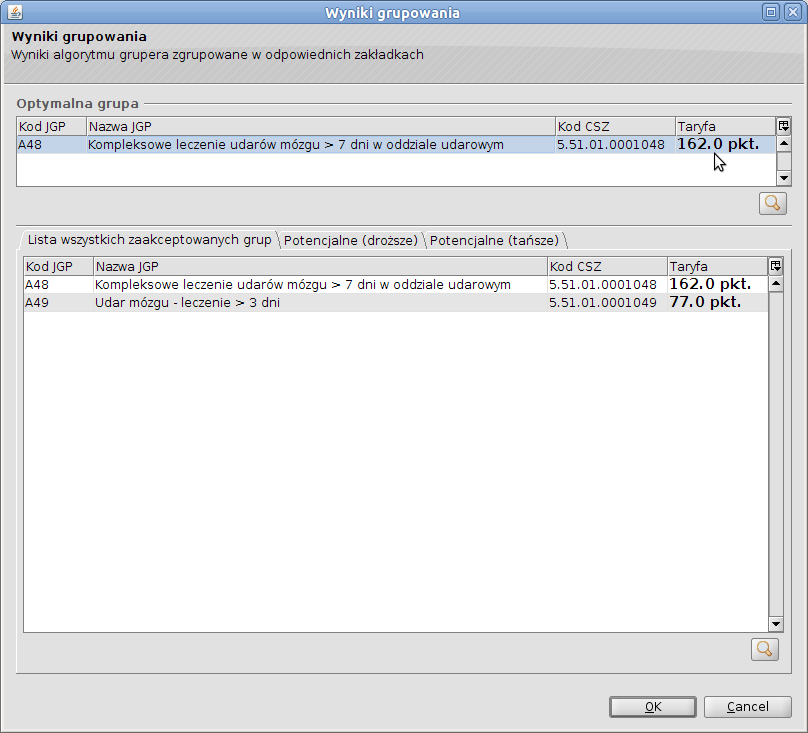
\includegraphics[scale=0.4]{images/gruper15}
\caption[Widok grupera]{Wyniki grupowania - Lista wszystkich zaakceptowanych grup.}
\label{img:gruper15}
\end{figure}

Wybrana zostaje grupa ,,A48 - Kompleksowe leczenie udarów mózgu > 7 dni w~oddziale udarowym''. Zoptymalizowany koszt leczenia to 162 jednostki punktowe.

%---------------------------------------------------------------------------

\section{Testy integracyjne}
\label{sec:testyIntegracyjne}

Dobrą praktyką zwiększającą współczynnik jakości oprogramowania jest wysokie pokrycie kodu w~testach. Zdecydowano się zatem napisać testy integracyjne klasy JGPService. Stworzono klasę ,,JGPServiceTest'', której zadaniem jest przetestowanie wszystkich głównych ścieżek algorytmu grupowania, gdzie testowana grupa wynikowa będzie pochodzić z~konkretnego warunku kierunkowego. Zatem poszczególne testy są napisane w~ten sposób, aby przetestować każdy z~możliwych 26 warunków kierunkowcyh A-Z.
Przykład przedstawiony w~sekcji \ref{sec:praktyczneUzycieSystemu} został również zaimplementwoany w~testach. Test ten sprawdza poprawne działanie systemu dla warunku kierunkowego E - ,,grupa zdefiniowana procedurą i~rozpoznaniem zasadniczym; może mieć dodatkowe warunki (czas hospitalizacji, wiek)''.
Dla testów integracyjnych przygotowana została testowa baza wiedzy. Przebieg testu jest następujący: ustalane są dane epizodu, uruchamiany jest mechanizm wnioskowania. Następnie sprawdzane są wyniki. Testowana jest poprawność wyników z~listy zaakceptowanych kodów oraz z~listy niezaakceptowanych kodów, wraz z~testami zgodności powodów niezaakceptowania z~wartościami oczekiwanymi.
Kod przykładowego testu integracyjnego zawiera listing \ref{java_test}.

\newpage
\begin{lstlisting}[language=Java,caption={Test integracyjny sprawdzający warunek kierunkowy ,,E''.},label=java_test]
@Test
public void testGrouperE() {
    Episode episode = createTestEpisode(new String[]{"G08"}, new String[]{"88.714"}, 7, 75);
    //run grouper
    JGPGroupResult result = jgpService.group(episode);
    //test accepted
    Assert.assertEquals(1, result.accepted().size());
    JGPResult acceptedJGP = result.accepted().get(0);
    Assert.assertEquals(77.0, acceptedJGP.getValue(), 0.0);
    Assert.assertEquals("A49", acceptedJGP.getJgp().getCode());
    //test NOT accepted
    Assert.assertEquals(1, result.notAccepted().size());
    JGPResult notAcceptedJGP = result.notAccepted().get(0);
    Assert.assertEquals(162.0, notAcceptedJGP.getValue(), 0.0);
    Assert.assertEquals("A48", notAcceptedJGP.getJgp().getCode());
    HospitalReason hospReason = notAcceptedJGP.reasons(HospitalReason.class).get(0);
    Assert.assertEquals(7, hospReason.required().getOver().intValue());
    Assert.assertEquals(TimeUnit.DAY, hospReason.required().getTimeUnit());
}
\end{lstlisting}

